\documentclass[11.5pt, twoside, a4paper]{article}
\usepackage{graphicx, amssymb, amsmath, amsthm, xfrac, mathabx, upgreek, fancyhdr, float, underscore, url}
\usepackage[margin=2cm]{geometry}
\usepackage[section]{placeins}
\setcounter{section}{-1}

\begin{document}

\title{Project Proposal: Underwater Robot for Fish Farms}
\author{Chanelle Lee}
\date{\today}
\maketitle

\section{Introduction}
This project aims to be part of wider work towards a prototype robotic platform for inspecting and cleaning nets underwater on commercial fish farms. Specifically, this robotic platform would be able to;
\begin{enumerate}
\item move autonomously about the net,
\item perform net inspection tasks,
\item clean the net of fouling, and
\item monitor fish.
\end{enumerate}
The time scale of this project is insufficient to tackle all of these problems and so the second has been chosen as the main aim of this project.

\section{Aims and Objectives}
As discussed this project will concentrate the performance of net inspection tasks of an underwater net cleaning robotic platform. The three aims of these inspection tasks, and the project objectives for each, are:
\begin{enumerate}
\item Identify damage to the net.
\begin{itemize}
\item Study image processing techniques for locating a net within an underwater image.
\item Develop an algorithm for detecting damage to the net.
\end{itemize}
\item Identify and quantify biofouling on the net.
\begin{itemize}
\item Study methods of identifying biofouling. %need to be more specific here
\item Study methods of quantifying biofouling.
\item Create software to identify biofouling within the image, and quantify the magnitude.
\end{itemize}
\item Recognise specific species of biofouling on the net.
\begin{itemize}
\item Study visual differences between types of biofouling, with emphasis on more harmful types.
\item Study classification methods.
\item Create software to recognise different species, specifically warning if recognise harmful species.
\end{itemize}
\end{enumerate}
All of these aims will be tested against images from fish farms and an experimental tank setup with real samples of netting, where the levels of biofouling and the quality of the water will be varied to test performance. If time allows, further work will be done to use the software developed here for locating the net and biofouling to create a simple navigational system for an AUV.

\section{Motivation}

Aquaculture is an increasingly important industry to Scotland, helping to create `sustainable economic growth in rural and coastal communities' \cite{ScotAqua} and is the world's third largest supplier of Atlantic Salmon. One important challenge to be tackled in aquaculture is the issue of biofouling; the colonisation of marine algae and animals on submerged components of cages and nets \cite{fitridge2012impact}. Biofouling of nets and cages has four main harmful effects \cite{fitridge2012impact, beveridge2008cage, Crown}:
\begin{itemize}
\item Restriction of water exchange from the occlusion of the netting mesh, which leads to lower dissolved oxygen (DO) levels and a build up of excess feed and waste. 
\item Cage deformation and structural fatigue from the extra weight and hydrodynamic forces upon the net.
\item Disease risk as fouling communities can act as reservoirs for pathogens and parasites.
\item The escape of stock due to net damage.
\end{itemize}
These all have a significant impact on the profitability of aquaculture through the loss of stock and net replacement and its removal is `expensive and labour-intensive, accounting for $20+\%$ of the market price of produce' \cite{Crown}. 

Traditional methods of biofouling removal include antifoulant paints, biological control and physical cleaning both in and out of the water. Toxic antifoulant paints have in the past been favoured as they are `more economical than manual cleaning' \cite{braithwaite2004marine}; the paint works by leaching biocides, such as copper, preventing fouling organisms from gaining a foothold on the net surfaces with treatments generally providing six months of protection \cite{beveridge2008cage}. However, reports that `copper levels in UK waters may be having an ecological effect' are raising concerns about the possible `long-term adverse effects in the environment' of antifoulants and in response their use is being phased out in the UK and across Europe. \cite{fitridge2012impact,braithwaite2004marine} Biological control of fouling, the inclusion of other species who feed on fouling organisms, has been suggested as the natural way to combat fouling, but it has been found to be `operationally impractical' \cite{Crown} and can lead to net damage and aggression against the stock species \cite{beveridge2008cage}. Physical cleaning of nets usually requires their removal from the water, then manual scrubbing with brushes and the use of pressurized water to remove the fouling; however, not only is this `tedious and labour-intensive' \cite{braithwaite2004marine}, but frequent handling and washing can damage nets and net changes cause unnecessary stress to the fish through handling and disruptions to feeding schedules \cite{Crown,fitridge2012impact}. In situ cleaning, normally performed by trained divers, negates the need to remove the net from the water, mitigating the harmful effects upon both net and fish; however, it is expensive and inefficient. Clearly, the high costs of physically cleaning nets are prohibitive and so it is performed relatively infrequently; this can lead to build ups of fouling, which can harbour harmful algae, bacteria, viruses and parasitic eggs and also allows net damage to go unchecked. Damage to nets is the `dominant means of reported escape for fish from Norwegian aquaculture' with two in three of all fish escapes being due to holes in netting \cite{jensen2010escapes} and fish escapes from cage farms not only represent an economic loss for the farmer, but also have many negative repercussions on the wild fish population \cite{mcdowell2002stream,jensen2010escapes}. Recently, the industry has been investigating the use of silicone-based foul-release coatings developed for marine vessels, which aim at `reducing or preventing the adhesion of fouling' \cite{fitridge2012impact}, as a non-toxic alternative to traditional antifoulant paints. Although their use relies upon the velocity of ships to dislodge the fouling, they would make the fouling easier to clean from netting and so many sources are recommending a move towards `foul-release coatings combined with in situ cleaning' \cite{Crown}. 

In recent years, many remotely operated underwater vehicle (ROV) systems of in situ net cleaning are emerging \cite{AKVA, MIC, Yanmar}, most using high pressurised jets of water to remove the fouling from the net. However, all of these still require at least one human operator to control the movement of the ROV and so they are still limited in their frequency of deployment. If the current ROVs systems could attain autonomy they would be able to continually clean and inspect the net with no need for a human operator; any damage or indications of parasites or disease could be discovered promptly, allowing fish farmers to then allocate more valuable resources, such as the time of trained divers, to remedial action, as opposed to wasting it on routine inspections. In order to do this it would need the ability to identify the net itself, and any biofouling or damage.  It has also been observed that there can be substantial spatial variations in the amount and types of biofouling within a cage system \cite{fitridge2012impact,hodson1997biofouling} and so in order to use resources efficiently a method of quantifying the amount of fouling would be needed. In addition, there is currently little data about biofouling and a way of monitoring could aid efforts to remove and even prevent it.

In summary, the main limitations of the state-of-the-art are the adverse environmental repercussions and that the dependency upon human labour restricts frequency of deployment or renewals. In an industry where regular inspections and cleaning can so dramatically improve profits and stock condition, it is clearly beneficial for a solution to perform both of these tasks, and to do so on a continuous basis.

\section{Literature Review}

This literature review will first briefly look at current state-of-the-art in-situ net cleaners. Then, in light of the limitations of these discussed above, the rest of the review will focus on current computer vision techniques which could help give autonomy to current net cleaners.

\subsection{In Situ Mechanical Net Cleaners}

One of the first instances of a mechanial in-situ net cleaner is \cite{hodson2000biofouling} in 1996, where it is proposed as way to allow longer periods of net immersion and so mitigate some of the costs and labour involved in on-shore cleaning. The cleaner comprised of four pairs of contra-rotating brushes and was attached to the handrail of the cage. Problems faced included; poor efficacy of the cleaner as the brushes has limited contact with the netting, a compromise was needed between brushing severity and the prevention of damage to netting, and the large amounts of debris created which could irritate fish or enable rapid recolonisation or regrowth. With the future introduction of foul-release silicon coatings the first two will become lesser issues; however, there is definitely a need for a debris removal system. 

\begin{figure}
\begin{center}
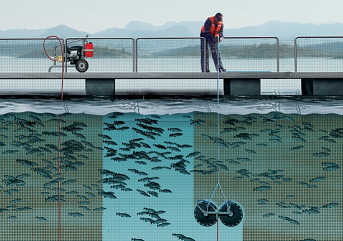
\includegraphics{cleaner.png}
\caption{Net cleaning system \cite{AKVA} \label{fig:cleaner}}
\end{center}
\end{figure}


There are now in situ net cleaners on the market \cite{Yanmar,AKVA,MPI,Hughesbrochure,MIC} and they have approached the problems raised by \cite{hodson1997biofouling} in a variety of ways. All \cite{AKVA,Hughesbrochure,MPI} use water ejectors to keep the cleaner pushed up against the net for more effective cleaning, while \cite{Yanmar} uses crawler belts and wheels to keep in contact with the net. Most use pressurised water to remove fouling, but \cite{MIC} is the only one found to use vacuum based net cleaning to remove the harmful debris. All of these cleaners appear very effective at cleaning biofouling; however, they still all require human operation, whether that is using a crane on a boat \cite{AKVA} or mounted on an ROV \cite{Hughesbrochure}. The next logical step then is to make these cleaners fully autonomous; this would reduce labour involved to maintenance, and would mean that the net would be constantly cleaned and inspected.

\subsection{Net Damage Detection}

Searching the literature has resulted in only a single source \cite{jakobsen2011automatic} concerning fish-cage net damage detection. That source is a masters thesis describing a micro-ROV with a fisheye camera to test the concept of automatic net inspection underwater and is a particularly useful paper as tests were carried out in situ at a fish farm. Two main methods were used to separate the foreground from the background within the images; segmentation through thresholding and edge detection. Thresholding was applied to all six channels in the RGB and HSV colour model and the red channel was found to perform best. An algorithm was used to set the threshold through the use of histograms and, in order to account for the change of lighting within the image, it was applied separately to sub blocks of the image. The use of the Canny Edge Detector was also investigated as a method of separating the image and when converted into a binary mask using a simple flooding algorithm the results were similar to those achieved through thresholding. Variations on the Hough transform were applied after the Canny Edge Detector to see if it could help with the sparseness of the detected edges; however, tests showed they either added no additional information, or added too much and would potentially add lines where there were none, not ideal when the aim is to detect breaks in the mesh. Experiments in situ at a fish farm showed thresholding to be the superior method over Canny Edge Detection, even in areas of high algae growth. Unfortunately, no more discussion or evidence is given as to the differences in performance of these two methods.  

\begin{figure}
\begin{center}
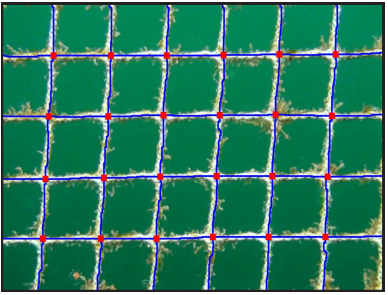
\includegraphics{Lines.png}
\caption{Figure 5.12 showing the results of the line detection algorithm after using a threshold on the red channel. \cite{jakobsen2011automatic} \label{fig:lines}}
\end{center}
\end{figure}

 
The use of stereo-photography in \cite{svane2006test} could provide information about the distance of the robot from the net, which could be used to keep the robot at a uniform distance for inspection in the absence of a frame or rig. It could also give a target for the control of any grippers or cleaning tools the robot might have; however, the movement of the net in the current could render this method of distance measurement unreliable. A different method of sensing the distance to the net is explored in \cite{jakobsen2011automatic}; a laser module consisting of two laser line generators. These laser lines can then be seen on the mesh and the distance between them can be calculated and from that the distance between the ROV and the net can be calculated. The use of laser lines was chosen over time of flight lasers or triangulation mainly because they both need to hit precisely the right area, but the edge of the net is narrow and so they would lack reliability. In test runs at a fish farm the laser module was found to be `robust with regards to distance, angle between ROV and net, algae growth, and rapid movements' \cite{jakobsen2011automatic} as long as it was within 60cm of the net. 

Detection of net damage is not implemented in \cite{jakobsen2011automatic} due to trouble acquiring footage of damage on which to test the software; however, it is suggested as the logical next step for further work and some methods are discussed. There is no indication that this further work has yet been done, and so this would make a good initial starting place for this project. 


\subsection{Biofouling Detection and Quantification}
The classic method for quantifying biofouling of fish-cage netting was to remove fouled netting from the water and then weigh it \cite{hodson1995situ}; however, this is obviously not a suitable method for this project. In \cite{hodson2000biofouling} the idea of using image analysis to quantify net fouling is first suggested and a method of quantifying net fouling in terms of mesh occlusion is given and as mesh occlusion is arguably the most detrimental effect of biofouling \cite{beveridge2008cage,fitridge2012impact,braithwaite2004marine}, this would provide a pertinent measurement for the amount of fouling.  Photographs were taken in situ with a single Nikonos-V camera and alterations to the environment were a single strobe light and a blue backing sheet to increase background contrast. The use of an artificial background is also found in \cite{braithwaite2007biofouling,edwards2015effectiveness} and this gives some cause for concern as to whether the method will be effective without the contrasting background. On the other hand, \cite{guenther2010development,svane2006test} all make no mention of using an artificial background, or that their results suffered by not having one. Although most studies \cite{braithwaite2007biofouling,guenther2010development,edwards2015effectiveness,gansel2015drag} only used a single camera, \cite{svane2006test} used two Nikonos V cameras to produces stereo-photographs giving a three-dimensional view of the net which could prove useful as an additional method of observing fouling; however, as no image analysis methods are discussed it can be inferred that the images were analysed manually, meaning caution should be had when approaching this method of image acquisition. Unfortunately, only \cite{guenther2010development} mentions the distance from the netting at which photographs were taken; the intial set up had the camera 12cm away from the netting, but modifications were made so that the camera was at a distance of 38cm from the net to `obtain an increase field of view'. This will be an important consideration for the project and will depend upon the AUV cleaner design and a trade off between other criteria. The field of view will need to be large enough to gather sufficient data, but, depending on the mesh size, this could lead to a very dense image, which require more computational power to analyse. Furthermore, by taking images closer to the net, illumination and turbidity are less of a problem due to the greater control of the scene that is within the field of view at any given time.

As most of the papers reviewed only discuss their method of biofouling quantification as a discussion of their testing set up for experiments, many lacked details with regards to their image processing methods. \cite{braithwaite2007biofouling} simply states the use of the software package `Image-Pro Plus 45' and the use of a written for purpose `macro-instruction'. \cite{hodson1995situ} used IDRISI, now called TerrSet, an `integrated geospatial software system' \cite{TerrSet} by Clark Labs. Segmentation by thresholding was used by \cite{guenther2010development,gansel2015drag,jakobsen2011automatic} to separate foreground and background in the images. Both \cite{guenther2010development} and \cite{jakobsen2011automatic} agree that the red channel was the most effective, but, despite following \cite{guenther2010development}, \cite{gansel2015drag} decided to use the luminance channel. As \cite{gansel2015drag} was working with a highly artificial environment compared to \cite{guenther2010development,jakobsen2011automatic} it is likely that the red channel would provide the better results for this project; however, it will be worth investigating due to the changeable nature of the environment. Only \cite{jakobsen2011automatic} has run these image processing methods in real time and even then a laptop was used, as the aim is to implement on a UAV any software would have to run in real time and with the limited computing power of a UAV.

\begin{figure}
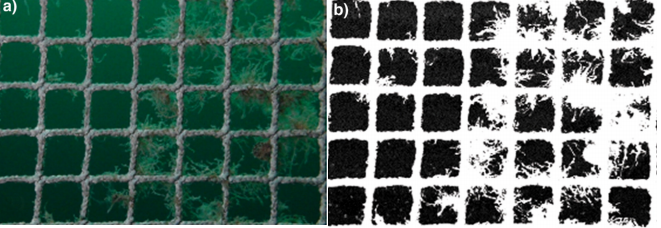
\includegraphics[width=\linewidth]{FoulingNet.png}
\caption{Example of an in situ photograph before and after image processing \cite{guenther2010development} \label{fig:foulingnet}}
\end{figure}


\subsection{Biofouling species recognition}

This aim of the project is perhaps the least supported by the literature. All reviews of the impacts of biofouling \cite{beveridge2008cage,braithwaite2004marine,fitridge2012impact} state that it can harbour parasites and disease harmful to fish, but nothing is mentioned about which types of fouling are indicative of this and so should be watched for. Biofouling studies express some interest in the composition of fouling and \cite{hodson1995situ} mentions that some fouling could be identified through colour. Identification from photographs alone \cite{edwards2015effectiveness,guenther2010development} was only completed manually by a human expert and even then identification to a species level was not possible. This all suggests that further research is necessary outside of biofouling studies to investigate whether the identification of biofouling using image analysis is possible to a useful level.

\subsection{Discussion}

To surmise, most of the literature discussed has only been used to identify and quantify biofouling for scientific studies with the image processing performed ex-situ. This project aims to be the first to move these methods in-situ and much of the work involved will concern evolving the methods to deal with these more challenging conditions. It will begin by replicating the work of \cite{jakobsen2011automatic}, developing the net damage detection algorithm mentioned in further work and then aims to integrate the biofouling quantification methods mentioned in \cite{hodson1995situ,guenther2010development}. Then there will be an investigation as to whether available image analysis techniques are able to identify biofouling in-situ, and if this proves possible the project aims be the first to apply them.

\section{Risk Register}

\begin{table}[h]
\centering 
\begin{tabular}{|p{4.5cm}|p{5cm} |c |c| c|} \hline
Risk & Mitigation & Likelihood & Impact & Score \\ [0.5ex] 
\hline 
Unable to acquire netting samples. & Ask for netting samples early so there is time to try different sources. & 2 & 3 & 6\\
\hline
Issue with testing tank rendering it unusable. & Allow flexibility so testing can be performed in a different tank. & 1 & 2 & 2\\
\hline
Unable to travel and meet fish farmers. & Utilise alternative communication methods, such as Skype or email. & 2 & 1 & 2\\
\hline
\end{tabular}
\label{table:risks} 
\caption{Risk Register} 
\end{table}


\section{Gantt Chart and Resources}

\subsection{Resources}

The necessary resources required for this project include:
\begin{itemize}
\item Netting with varying levels of biofouling and wear.
\item Test tanks with the ability to control water quality.
\item Test rig attachable to the tank able to support net and camera.
\item Underwater camera. (Nikonos-V or  SONY HDR-SR12 handycam are used in the literature.)
\item Stereo-camera. (Water-proof.)
\item Laser module. (Either replicated from \cite{jakobsen2011automatic} or a suitable substitute.)
\item Strobe-lights.
\item Matlab with the Image Processing ToolBox.
\item A robotic platform such as an Arduino.
\end{itemize}

\begin{figure}
\begin{center}
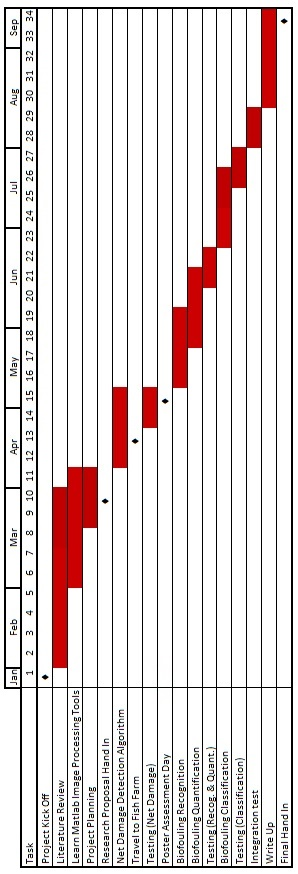
\includegraphics{Gantt.jpg}
\caption{Gantt chart showing project time line and important events \label{fig:gantt}}
\end{center}
\end{figure}

\bibliographystyle{unsrt}
\bibliography{FishProject}{}


\end{document}